\documentclass[11pt]{report}
\usepackage{fullpage}
\usepackage{graphicx}
\usepackage{psfig}
\usepackage{amsmath}
\usepackage{times}
\usepackage{cite}
\usepackage{url}
\usepackage{longtable}

\newcommand{\comment}[1]{\textit{\small {#1}}}
\newcommand{\cpp}{C\texttt{++}\ }
\newcommand{\tcl}{\textsc{Tcl\ }}
\newcommand{\ProtoMol}{\textsc{ProtoMol}}
\newcommand{\SamdII}{\textsc{Samd 2\ }}
\newcommand{\MOLLY}{\textsc{MOLLY\ }}

\newcommand{\tempstart}{\texttt{<}}
\newcommand{\tempend}{\texttt{>}}
\newcommand{\rij}{\mbox{r$_{ij}$}}
\newcommand{\rik}{\mbox{r$_{ik}$}}
\newcommand{\vrij}{\mbox{$\vec{r}_{ij}$}}
\newcommand{\Si}[1]{\mbox{Si$_{#1}$}}
\newcommand{\Vr}[1]{\mbox{$\vec{r}_{#1}$}}
\newcommand{\Vx}[1]{\mbox{$\vec{x}_{#1}$}}
\newcommand{\Vv}[1]{\mbox{$\vec{v}_{#1}$}}
\newcommand{\hatr}[1]{\mbox{$\hat{{r}_{#1}}$}}
\newcommand{\hatv}[1]{\mbox{$\hat{{v}_{#1}}$}}
\newcommand{\AbsVr}[1]{\mbox{$\left| \vec{r}_{#1} \right| $}}
\newcommand{\AbsVv}[1]{\mbox{$\left| \vec{v}_{#1} \right| $}}
\providecommand{\textinmath}[1]{\mbox{#1}}
\providecommand{\ttsmall}[1]{\texttt{\small\mbox{#1}}}

\title{\ProtoMol\ Version 2.0.3 - Quick Reference}

\begin{document}
\maketitle

\chapter{Introduction}
Molecular Dynamics (MD) describes a molecular system as a function of
time based on integration of equations of motion. 
 The most computationally expensive part is the force
calculation at every time step.  There have been many implementations to
solve one given problem very efficiently, but they usually lack
flexibility when trying to implement new methods or approaches to
solve the problem.  What \ProtoMol\ provides is a generic,
object-oriented component framework for MD simulations.  To meet these
high performance expectations, \ProtoMol\ uses cell algorithms, grid
techniques and well-optimized libraries for the most
computationally expensive forces.  The design of \ProtoMol\ also
includes parallelization, based on components to distribute the work
and data.  The approach follows an incremental and partial
parallelization scheme, which allows the developer to start with a
sequential implementation and then do step by step parallelization. \\


The overall framework of \ProtoMol\ is designed for non-bonded, bonded,
short-range and long-range forces for systems with tens of thousands
of atoms representing water and several large molecules.  It is
designed for high flexibility, ease in extension and maintainence, and
high performance demands.

%%%%%%%%%%%%%%%%%%%%%%%%%%%%%%%%%%%%%%%%%%%%%%%%%%%%%%%%%%%%%%%%%%%%%%%%%
\section{Useful Features}

%%%%%%%%%%%%%%%%%%%%%%%%%%%%%%%%%%%%%%%%%%%%%%%%%%%%%%%%%%%%%%%%%%%%%%%%%

%%%%%%%%%%%%%%%%%%%%%%%%%%%%%%%%%%%%%%%%%%%%%%%%%%%%%%%%%%%%%%%%%%%%%%%%%
\subsection{Force field}

\ProtoMol\ supports force fields in the same format that CHARMM uses,
including bonded interactions between groups of 2 (bonds), 3 (angles),
and 4 (dihedrals and impropers) atoms, as well as electrostatic and
van der Waals nonbonded interactions.

%%%%%%%%%%%%%%%%%%%%%%%%%%%%%%%%%%%%%%%%%%%%%%%%%%%%%%%%%%%%%%%%%%%%%%%%%
\subsection{Multiple time-stepping}

Multiple time-stepping is a useful technique for cost reduction of
calculating long-range electrostatic forces.  The idea behind multiple
time-stepping is to compute at every timestep bonded, van der Waals
and short-range electrostatic forces, while computing long-range
electrostatic forces less often.  Overtime this will result in
improved efficiency because the cost for computing electrostatic
interactions will be amortized over the number of timesteps to be run
in the simulation~\cite{BHAN01}.

%%%%%%%%%%%%%%%%%%%%%%%%%%%%%%%%%%%%%%%%%%%%%%%%%%%%%%%%%%%%%%%%%%%%%%%%%
\subsection{Comparison of force algorithms}

\ProtoMol\ is able to compare forces measuring the error and the time;
e.g. an exact algorithm with a fast approximation.

%%%%%%%%%%%%%%%%%%%%%%%%%%%%%%%%%%%%%%%%%%%%%%%%%%%%%%%%%%%%%%%%%%%%%%%%%
\subsection{Ability to interact with VMD}

VMD is a program developed by the University of Illinois that is used
for displaying large biomolecular systems in three
dimensions. \ProtoMol\ is conveniently able to interact with this
useful program. For more information, see:\\
\\
\ttsmall{http://www.ks.uiuc.edu/Research/vmd}

%%%%%%%%%%%%%%%%%%%%%%%%%%%%%%%%%%%%%%%%%%%%%%%%%%%%%%%%%%%%%%%%%%%%%%%%%
\subsection{Ability to run on parallel machines}

The most computationally expensive part of an MD simulation is force
evaluation between atoms.  Because so much computing power is required
for the force evaluation of large systems, {\it i.e.,} 5000 atoms or
more, the ability to run MD simulations on parallel machines will hold
a large advantage with regard to speed.  \ProtoMol\ has been designed
to take advantage of parallel computing in running MD simulations.

%%%%%%%%%%%%%%%%%%%%%%%%%%%%%%%%%%%%%%%%%%%%%%%%%%%%%%%%%%%%%%%%%%%%%%%%%
\subsection{Installation}
Please follow the README file under protomol directory for installation 
instructions.

%%%%%%%%%%%%%%%%%%%%%%%%%%%%%%%%%%%%%%%%%%%%%%%%%%%%%%%%%%%%%%%%%%%%%%%%%


%%%%%%%%%%%%%%%%%%%%%%%%%%%%%%%%%%%%%%%%%%%%%%%%%%%%%%%%%%%%%%%%%%%%%%%%%
\subsection{Licensing}
\ProtoMol\ is a free software, available under GNU general public license(GPL)
\footnote{http://www.gnu.org/licenses/licenses.html\#GPL}. Please cite
\cite{Matt04} if you are using \ProtoMol\ for your research.

\chapter{Getting Started}

This chapter will introduce the commands and settings needed to run
\ProtoMol.  Included are the exact formats of the command line on a
UNIX / Linux machine and the configuration file containing all initial
information to run the MD simulation.  In Chapter 4 we will show three
sample configuration files.

%%%%%%%%%%%%%%%%%%%%%%%%%%%%%%%%%%%%%%%%%%%%%%%%%%%%%%%%%%%%%%%%%%%%%%%%%
\section{Command Line}

The MD application of the \ProtoMol\ framework has conveniently been
named \ttsmall{protomol}.  At a UNIX / Linux prompt, a user types
\ttsmall{protomol} followed by an alternating list of keywords and
arguments (see chapter \ref{sec:keywordsection} for a list of keywords).  Thus, the
general format for the \ProtoMol\ execution command is the following:\\
\\
\ttsmall{protomol [--keyword1}
{\it value1}
\ttsmall{] [--keyword2} 
{\it value2}
\ttsmall{] [--keyword3}
{\it value3}
\ttsmall{] .......}\\

{\it Note that keywords must be preceded by two dashes, where a value
can be a list of values - e.g. for the keyword CellBasisVector1.  Also
note that any keyword-value pair specified on the command line
overrides any according pair in the configuration file.}\\


The user may also specify any of these keywords and values in the
configuration file that he or she is using.  The
exact pathname of the configuration file being used for running
\ProtoMol\
must be
specified on the command line. For example, the configuration file
can be specified one of the following ways: \\
\ttsmall{protomol [--config] <pathname/myconfigfilename>
......}\\

{\it The }\ttsmall{--config} {\it keyword can be omitted
if the configuration file is the first thing specified.}\\

\ttsmall{\indent protomol ..... --config <pathname/myconfigfilename> .....}

%%%%%%%%%%%%%%%%%%%%%%%%%%%%%%%%%%%%%%%%%%%%%%%%%%%%%%%%%%%%%%%%%%%%%%%%%
\subsection{Help Option}

A user may type one of the following two possibilities at a UNIX / Linux
prompt for help with the \ProtoMol\ command line: \\
\begin{enumerate}
\item \ttsmall{protomol -h}
\item \ttsmall{protomol --help}
\end{enumerate}

%%%%%%%%%%%%%%%%%%%%%%%%%%%%%%%%%%%%%%%%%%%%%%%%%%%%%%%%%%%%%%%%%%%%%%%%%
\section{Simple GUI}

In oder simplify the usage of \ProtoMol\ (i.e., on Windows) you may
use the simple perl/Tk GUI
front-end \texttt{TkProtomol.pl}. The script is located
under \texttt{protomol/tools}, and has a simple editor and plotter. 
\begin{figure}[htb]
        \begin{minipage}[htb]{8cm} 
   \centerline{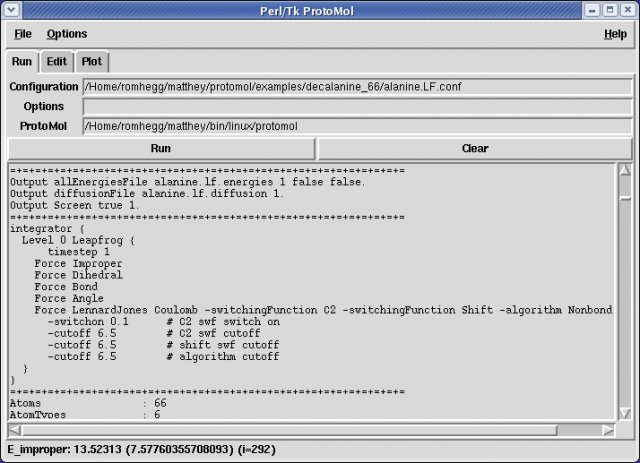
\includegraphics[width=7.5cm]{tkprotomol.jpg}}

        \end{minipage} 
        \hfill
       \begin{minipage}[htb]{8cm}
   \centerline{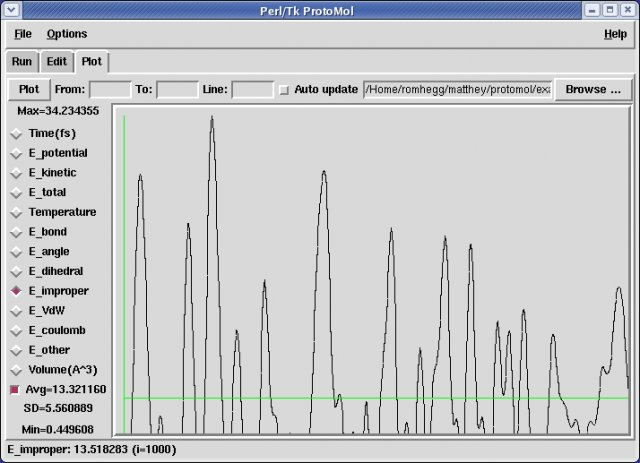
\includegraphics[width=7.5cm]{tkprotomol_plot.jpg}}
        \end{minipage}
        \caption{Simple perl/Tk GUI front-end. \label{fig:tkprotomol}}
\end{figure}

%%%%%%%%%%%%%%%%%%%%%%%%%%%%%%%%%%%%%%%%%%%%%%%%%%%%%%%%%%%%%%%%%%%%%%%%%
\section{Configuration File}

The configuration file is a text file containing a collection of
keyword-value pairs specifying the simulation configuration, I/O files
and formats, and the definition of the integrator scheme. 

%%%%%%%%%%%%%%%%%%%%%%%%%%%%%%%%%%%%%%%%%%%%%%%%%%%%%%%%%%%%%%%%%%%%%%%%%

\subsection{Format of \ProtoMol\ keywords in the configuration file}

The configuration file format for \ProtoMol\ is quite simple, making it
convenient for creation and modification of the file.  The advantage
of straightforward modification of the configuration file is that the
user can very easily switch between running the same molecule under
different initial conditions, or even switch to a different molecule
without much trouble.  The general format for a \ProtoMol\
configuration file is a list of keywords and values, with whitespace
between each keyword and value and a newline between each new
keyword-value pair:
\newline

{\bf keyword1}{\it \indent    value1}\\
{\bf \indent keyword2}{\it \indent   value2} \# comment\\
\indent \# comment\\
{\bf \indent keyword3}{\it \indent   value3}\\
{\bf \indent \indent \indent \indent  .}\\
{\bf \indent \indent \indent \indent  .}\\
{\bf \indent \indent \indent \indent  .}\\
\newline

{\it A list of \ProtoMol\ keywords, possible values and defaults can
  be found in section \ref{sec:keywordsection}, or type\\
  \ttsmall{protomol -m --keywords}} .

%%%%%%%%%%%%%%%%%%%%%%%%%%%%%%%%%%%%%%%%%%%%%%%%%%%%%%%%%%%%%%%%%%%%%%%%%
\subsection{Format of the integrator and their arguments}

In addition to the keyword-value pairs in the configuration file, one
must set up an integrator in the following manner:

{\bf Integrator \{}\\
{\bf \indent \indent level N-1} \tempstart integrator type\tempend  {\bf \{} \# MTS integrator \\
{\indent \indent \indent \tempstart integrator arguments\tempend }
{\it (These will differ depending on the integrator type). }\\
{ \indent \indent \indent \tempstart integrator forces\tempend }
{\it (These are all optional). }\\
{\bf \indent \indent \} }\\
{\bf \indent \indent .}\\
{\bf \indent \indent .}\\
{\bf \indent \indent .}\\
\\
{\bf \indent \indent level 0} \tempstart integrator type\tempend  {\bf \{} \# STS integrator\\
{\bf \indent \indent \indent .}\\
{\bf \indent \indent \indent .}\\
{\bf \indent \indent \indent .}\\
{\bf \indent \indent \} }\\
{\bf \indent \}}\\ 

Note that the order of definition for each level is not strict, but
\ProtoMol\ expects one definition for each level.

%%%%%%%%%%%%%%%%%%%%%%%%%%%%%%%%%%%%%%%%%%%%%%%%%%%%%%%%%%%%%%%%%%%%%%%%%
\subsubsection{Integrator Types}

\begin{itemize}
\item Multiple Timestep Integrators (MTS)
  \begin{enumerate}
  \item {\bf BSplineMOLLY}
  \item {\bf EquilibriumMOLLY}
  \item {\bf HybridMC} {\it (Hybrid Monte Carlo Integrator)}
  \item {\bf Impulse} {\it (Verlet-I/r-RESPA)}
  \item {\bf ShadowHybridMC} {\it (Shadow Hybrid Monte Carlo Integrator)}
  \item {\bf Umbrella}	
  \end{enumerate}
\item Single Timestep Integrators (STS)
  \begin{enumerate}
  \item {\bf BBK}
  \item {\bf DMDLeapfrog} {\it (Self-consistent Leapfrog from Dissipative Particle Dynamics)}
  \item {\bf DihedralHMC }  
  \item {\bf DihedralLiftMC }  
  \item {\bf LangevinImpulse}
  \item {\bf Leapfrog }    {\it (Velocity Leap-Frog Integrator)}
  \item {\bf NPTVerlet}
  \item {\bf NoseNVTLeapfrog}
  \item {\bf PLeapfrog }    {\it (Position Leap-Frog Integrator)}
  \item {\bf PaulTrap }  
  \end{enumerate}
\item Alias
  \begin{itemize}
  \item HBondMOLLY : BSplineMOLLY
  \end{itemize}
\end{itemize}

The choice of what integrator to use in ProtoMol is largely determined by
the intended application. The main applications of molecular dynamics (MD)
are equilibration, dynamics proper (e.g., to compute transport properties
and autocorrelation functions), kinetics (e.g., to compute transition rates
between metastable states), and sampling (e.g., to compute thermodynamic
properties such as the free energy). 

Computation of dynamics is more stringent than the other applications of MD.
One should probably equilibrate a number of replicas from the desired
ensemble (NVT or NPT) and then run NVE simulations. For NVE simulation, the
standard integrator is the single time stepping Leapfrog. Usually the
velocity version is preferred. However, if one uses multiple time stepping,
the position version may be better. For solvated biomolecules the time step
used in leapfrog is typically 1$\,$fs, although the stability limit is
around 2.25$\,$fs. Using Shake (and optionally Rattle) to constrain bond
lengths to Hydrogen allow longer time steps by roughly a factor of 2. Other
tricks are used to use longer time steps, such as altering the mass of
Hydrogens, etc. 

Multiple time stepping (MTS) allows one to use longer time steps, although
the presence of nonlinear and linear resonances (at one third and one half
the fastest period in the system, cf. \cite{MaIS03}) significantly limits
the time steps available. The Verlet-I/r-RESPA/Impulse method can take long
time steps of 3.3$\,$fs without energy drift for very long times (several ns
of simulation). One can get even longer steps using either the Equilibrium
MOLLY \cite{IzRS99} or the Bspline-MOLLY \cite{Izag99} method. Long time
steps for unconstrained biomolecules of 6$\,$ fs have been reported,
although care is recommended if using time steps of 5$\,$ fs or more. One
should carefully analyze the time series of energy to see whether an
intolerable drift is occurring over the length of the simulation.

For equilibration or sampling in NVT, we recommend using the Langevin
Impulse method, which is exact for constant force. A good alternative is the
self-consistent Leapfrog method (DMDLeapfrog), which preserves linear
momentum and therefore hydrodynamics properties. We discourage the use of
extended Hamiltonian methods such as Nose-Hoover (NoseNVTLeapfrog), since
these are frequently not ergodic and have difficulty maintaining
equipartition \cite{Hamp0x}.
For equilibration in NPT, we have implemented the NPT Verlet method
(NPTVerlet). This is probably the best equilibration scheme in ProtoMol, but
it requires some fine tuning of the parameter scheme. Note that there are
currently no minimization schemes in \textsc{ProtoMol}. We recommend using
NAMD 2.5 for minimization if required. This will be alleviated soon.

For sampling from the canonical (NVT) ensemble, one can also use Hybrid
Monte Carlo methods to eliminate the systematic error due to discretization
error in MD, which is manifested as time step dependence of the averages
computed using MD. For small systems, Hybrid Monte Carlo is adequate. For
larger systems (upward of hundreds of atoms), Shadow Hybrid Monte Carlo is
the best choice. One has to choose a parameter $c$ that controls efficiency
and variance in observables, see \cite{IzHa04} and \cite{Hamp0x}.

Note that one can build a replica exchange protocol with ProtoMol - we
currently do it using scripting, but this will be soon incorporated into the
main code. This is a much more efficient way of sampling. 


%%%%%%%%%%%%%%%%%%%%%%%%%%%%%%%%%%%%%%%%%%%%%%%%%%%%%%%%%%%%%%%%%%%%%%%%%
\clearpage
\subsubsection{Integrator Argument Types}

\begin{enumerate}

\item {\bf BBK}
\begin{list}{~}
\item {\bf timestep} \tempstart length of step (float)\tempend
\item {\bf temperature} \tempstart Kelvin temperature (float)\tempend
\item {\bf gamma} \tempstart gamma (float)\tempend
\item {\bf seed} \tempstart random seed (integer)\tempend
\end{list}

\item {\bf BSplineMOLLY}
\begin{list}{~}
\item {\bf cyclelength} \tempstart length of cycle (integer)\tempend
\item {\bf BSplineType} \tempstart {short$|$long}\tempend
\item {\bf mollyStepSize} \tempstart stepsize used for MOLLY integrator \tempend
\end{list}


\item{\bf DihedralHMC}
\begin{list}{~}
\item {\bf cyclelength} \tempstart Length of cycle (integer)\tempend
\item {\bf temperature} \tempstart Kelvin temperature (in K)\tempend
\item {\bf randomCycLen} \tempstart Use a random adjustment to cyclelength (boolean) \tempend
\item {\bf dihedralsSet} \tempstart Flag to specify which dihedrals to move, if false then dihedrals chosen randomly (boolean)\tempend
\item {\bf dhmcDiSetFile} \tempstart The dihedral indices are to specified in this file (string) \tempend
\item {\bf anglesSet} \tempstart  (boolean)\tempend
\item {\bf dhmcAnSetFile} \tempstart (string) \tempend
\end{list}

\item{\bf DihedralLiftMC}
\begin{list}{~}
\item {\bf cyclelength} \tempstart Length of cycle (integer)\tempend
\item {\bf randomCycLen} \tempstart Use a random adjustment to cyclelength (boolean) \tempend
\item {\bf temperature} \tempstart Preferred system temperature (in K)\tempend
\end{list}

\item {\bf DMDLeapfrog}
\begin{list}{~}
\item {\bf timestep} \tempstart Size of each step (float)\tempend
\item {\bf iterations} \tempstart number of iterations (integer)\tempend
\item {\bf gamma} \tempstart gamma (float)\tempend
\item {\bf temperature} \tempstart Kelvin temperature (float)\tempend
\item {\bf seed} \tempstart seed to generate random numbers (integer)\tempend
\end{list}

\item {\bf EquilibriumMOLLY}
\begin{list}{~}
\item {\bf cyclelength} \tempstart length of cycle (integer)\tempend
\end{list}

\item {\bf HybridMC}
\begin{list}{~}
\item {\bf cyclelength} \tempstart length of cycle (integer)\tempend
\item {\bf randomCycLen} \tempstart Use a random adjustment to cyclelength (bool)\tempend
\item {\bf temperature} \tempstart Kelvin temperature (float)\tempend
\end{list}

\item {\bf Impulse}
\begin{list}{~}
\item {\bf cyclelength} \tempstart length of cycle (integer)\tempend
\end{list}

\item {\bf LangevinImpulse}
\begin{list}{~}
\item {\bf timestep} \tempstart length of step (float)\tempend
\item {\bf temperature} \tempstart Kelvin temperature (float)\tempend
\item {\bf gamma} \tempstart gamma (float)\tempend
\item {\bf seed} \tempstart random seed (integer)\tempend
\end{list}

\item {\bf Leapfrog}
\begin{list}{~}
\item {\bf timestep} \tempstart length of step (float)\tempend
\end{list}

\item {\bf NoseNVTLeapfrog}
\begin{list}{~}
\item {\bf timestep} \tempstart length of each step (float)\tempend
\item {\bf temperature} \tempstart preferred system temperature(in K)\tempend
\item {\bf thermal} \tempstart  heat bath coupling( 1.0:very strong, 0:none) (float)\tempend
\item {\bf bathPos} \tempstart history of the difference of system and heat bath (float)\tempend
\end{list}

\item{\bf NPTVerlet}
\begin{list}{~}
\item {\bf timestep} \tempstart length of step (float)\tempend
\item {\bf temperature} \tempstart Kelvin temperature (in K) \tempend
\item {\bf pressure} \tempstart (in  Bar) \tempend
\item {\bf omegaTo} \tempstart thermostat frequency\tempend
\item {\bf omegaTv} \tempstart volume thermostat frequency \tempend
\item {\bf tauP} \tempstart barostat time period \tempend
\end{list}

\item{\bf PaulTrap}
\begin{list}{~}
\item {\bf timestep} \tempstart length of step (float)\tempend
\item {\bf temperature} \tempstart Kelvin temperature(in K)\tempend
\item {\bf thermal} \tempstart (float)\tempend
\item {\bf bathPos} \tempstart (float)\tempend
\item {\bf bathVel} \tempstart (float)\tempend
\item {\bf scheme} \tempstart thermostat scheme {NVT$|$NVT\_zero$|$NVT\_ind$|$ 
NVT\_shell$|$NVT\_global$|$berendsen$|$berendsen\_zero \\
$|$berendsen\_ind$|$ 
berendsen\_shell$|$berendsen\_global} (string) \tempend

\item {\bf part} \tempstart  (float)\tempend
\item {\bf time} \tempstart  (vector)\tempend
\item {\bf t} \tempstart  (vector)\tempend
\end{list}

\item {\bf PLeapfrog}
\begin{list}{~}
\item  {\bf timestep} \tempstart length of step (float)\tempend
\end{list}

\item {\bf ShadowHMC}
\begin{list}{~}
\item  {\bf cyclelength} \tempstart length of step (float)\tempend
\item  {\bf randomCycLen} \tempstart Use a random adjustment to cycleLengthi (boolean) \tempend
\item {\bf temperature} \tempstart Preferred system temperature(in K)\tempend
\item {\bf order} \tempstart Desired order of approximation (4th or 8th)\tempend
\item {\bf c} \tempstart Parameter to specify divergence between shadow and total energy (float)\tempend
\end{list}

\item {\bf Umbrella}
\begin{list}{~}
\item  {\bf cyclelength} \tempstart length of step (float)\tempend
\end{list}


\end{enumerate}


%%%%%%%%%%%%%%%%%%%%%%%%%%%%%%%%%%%%%%%%%%%%%%%%%%%%%%%%%%%%%%%%%%%%%%%%%
\subsubsection{General Format of Integrator Forces}

{\bf force} \tempstart force1 type\tempend  \\
\indent \tempstart force1 arguments\tempend  \\
{\bf force} \tempstart force2 type\tempend  \\
\indent \tempstart force2 arguments\tempend  \\
{\bf force} \tempstart force3 type\tempend  \\
\indent \tempstart force3 arguments\tempend  \\
$\dots$\\
\textsc{ProtoMol} supports primarily forces defined by the CHARMM
forcefields (versions 19 and 27). There are some custom forces
available (haptic force, friction, gravitation, Paul Trap, external
field, external gravitation, Harmonic biasing force HarmDihedral,
magnetic dipole, etc.) and it is easy to add new forces. You can look
at the forces available in your copy of \texttt{ProtoMol} by running
\texttt{protomol -f}.

�

You can include forces at will in your integrator. A nice tutorial on
how to compose MTS integrators along with the forces is at
\url{http://www.nd.edu/~izaguirr/papers/m3paper.pdf}. �Some forces do
not have parameters. This is particularly the case of bonded forces:
angle, bond, dihedral, and improper. Nonbonded forces have several
parameters, which fall primarily in these categories:

�

\begin{itemize}

\item \textbf{Potential:} Primarily Coulomb or Lennard Jones.

\item \textbf{Algorithm:} This option refers to the algorithm used to
compute the sum of pairwise interactions. Depending on the boundary
condition and the potential, there are a number of algorithms:

\begin{itemize}

\item For both Lennard Jones and Coulomb in periodic and vacuum
boundary conditions, one can use cutoff computation
(\texttt{-algorithm NonbondedCutoff}) or direct computational of all
interactions (\texttt{-algorithm NonbondedFull})

\item For Coulomb computation one can use an $O(N)$ multigrid
summation (\texttt{-algorithm multigrid}) \cite{IzHM05}, both for
vacuum or periodic boundary conditions. This is an attractive
alternative to PME or Ewald, since it scales better in parallel.
Setting the parameters requires some knowledge, so we recommend using
the online recommender system \textsc{MDSimAid} at
http://mdsimaid.cse.nd.edu

\item For Coulomb one can also use PME (\texttt{-algorithm PMEwald})
or Ewald (\texttt{-algorithm FullEwald}).

\end{itemize}

\item \textbf{Switching function:} when using cutoff or MTS
integrators, one needs to bring the potential energy (and hence the
force) smoothly to zero to avoid discontinuities that destabilize the
integrators for MD. For LennardJones we recommend using a $C^2$
continuous switching function (\texttt{-switchingFunction C2}). For
Coulomb a $C^1$ switching function often suffices
(\texttt{-switchingFunction C1}). It is also easy to add switching
functions.

\item \textbf{Method specific parameters: } Some methods require
specific parameters, see the current force definitions accepted in
\texttt{ProtoMol} by running \texttt{protomol -f}.

\end{itemize}

�



%%%%%%%%%%%%%%%%%%%%%%%%%%%%%%%%%%%%%%%%%%%%%%%%%%%%%%%%%%%%%%%%%%%%%%%%%
\section{Required Parameters}
    
As mentioned earlier, the command line must contain either the full
pathname of the configuration file.  These are
the only restrictions specifically applied to the command line. \\
    
The following parameters MUST be specified on either the command line
or in the configuration file specified on the command line (you may
view Chapter 3 for a list of supported \ProtoMol\ files and their 
formats):
      
\begin{itemize}
  \item One of either an initial positions file in PDB or XYZ or Binary format.
    
  \item One of an initial velocities file in PDB or XYZ or Binary format,  or an initial temperature.

  \item A PSF topology file.
    
  \item A CHARMM Par parameters file.

  \item If the user specifies any specific output files that should be written, they must specify a filename.

  \item The number of steps for the simulation.

  \item A cubic cell manager and either vacuum or periodic boundary
  conditions.

  \item An integrator.

\end{itemize}

%%%%%%%%%%%%%%%%%%%%%%%%%%%%%%%%%%%%%%%%%%%%%%%%%%%%%%%%%%%%%%%%%%%%%%%%%
\chapter{\ProtoMol\ keyword and descriptions}
\label{sec:keywordsection}

\section{Input files}
\begin{center}
  \begin{longtable}{|p{4cm}|p{2cm}|p{9.5cm}|}
    \hline
    keyword & type & Description \\
	\hline
	posfile & 
	string & 
    Contains the full or relative pathname of the initial positions file.  \ProtoMol\ supports PDB, XYZ or Binary formatted position files.  \\\hline

	velfile & 
	string & 
    Contains the full or relative pathname of the initial velocities file.  Once again, \ProtoMol\ supports PDB, XYZ or Binary formats.  If no initial velocity file is specified, random velocities are generated based on the initial temperature and a seed that can also be specified. Therefore one of either the velfile, or temperature needs to be specified. A seed is optional.\\\hline

    psffile &
    string &
    Contains the full or relative pathname of the initial topology file in PSF format. \\\hline

    parfile / parameters &
    string &
    Contains the full or relative pathname of the initial CHARMM parameter file. \\\hline


  \end{longtable} 
\end{center}

%%%%%%%%%%%%%%%%%%%%%%%%%%%%%%%%%%%%%%%%%%%%%%%%%%%%%%%%%%%%%%%%

\section{Boundary Conditions}
\begin{center}
  \begin{longtable}{|p{4cm}|p{2cm}|p{9.5cm}|}
    \hline
    keyword & type & Description \\
    \hline

    boundaryconditions &
    string &
    \ProtoMol\ supports vacuum or periodic boundary conditions, specified with ``Vacuum'' or ``Periodic'', respectively. \\\hline

    cellbasisvector1 &
    x  y  z  (x, y, and z are floats) &
    Basis vector 1, for periodic boundaries\\\hline
                                                                                                
    cellbasisvector2 &
    x  y  z  (x, y, and z are floats) &
    Basis vector 2, for periodic boundaries\\\hline
                                                                                                
    cellbasisvector3 &
    x  y  z  (x, y, and z are floats) &
    Basis vector 3, for periodic boundaries\\\hline
                                                                                                
    cellorigin &
    x  y  z  (x, y, and z are floats) &
    Center of periodic cell, for periodic boundaries\\\hline



  \end{longtable}
\end{center}

%%%%%%%%%%%%%%%%%%%%%%%%%%%%%%%%%%%%%%%%%%%%%%%%%%%%%%%%%%%%%%%%%%

\section{Output Files}
\begin{center}
  \begin{longtable}{|p{4cm}|p{2cm}|p{9.5cm}|}
    \hline
    keyword & type & Description \\
    \hline

    dcdfile &
    string &
    Contains the full or relative pathname of the DCD trajectory file to be written, if desired.  \\\hline
                                                                                                
    dodcdfile &
    boolean  &
    Specifies if the user would like a DCD trajectory file to be written. \\\hline

    allenergiesfile &
    string &
    Contains the full or relative pathname of the energies file to be written, again if desired.  \\\hline
                                                                                                
    doallenergiesfile &
    boolean (default: true) &
    Specifies if the user would like an energies file to be written, with all energies (bond, angle, dihedral... whatever was forced in the integrator section) in one file. \\\hline

    allenergiesFileOutputFreq &
    integer (default: outputFreq) &
    Specifies the frequency of the energies file to be written, if desired.\\\hline

    allEnergiesFileCacheFreq  &
    integer (default: 1) &
    Specifies frequency in number of lines to flush the cache to
    file.\\\hline

    allEnergiesFileCacheSize &  
    integer (default: 0) &
    Specifies the minimal size of cached data to flush to file\\\hline

    allEnergiesFileCloseTime & 
    float (default: 1.0) &
    Specifies the minimal time interval between two writes to close the file temporarily\\\hline


    outputfreq &
    integer &
    Specifies the frequency in timesteps for the writing of energy
    data to the console and defines the default frequency for other
    outputs. \\\hline

    finpdbposfile &
    string &
    Contains the full or relative pathname of the final positions file in PDB format, if the user desires. \\\hline
                                                                                                
    dofinpdbposfile &
    boolean  &
    Specifies if the user would like a final PDB positions file to be written.  \\\hline

    xyzposfile &
    string &
    Contains the full or relative pathname of the positions trajectory file in XYZ format, once again if desired. \\\hline
                                                                                                
    doxyzposfile &
    boolean  &
    Specifies if the user would like an XYZ trajectory file for positions to be written. \\\hline
                                                                                                
    xyzposFileOutputFreq &
    integer (default: outputFreq) &
    Specifies the frequency of the XYZ trajectory file for positions to be written, if desired.\\\hline

    xyzvelfile &
    string &
    Contains the full or relative pathname of the XYZ velocities trajectory file, if desired.  \\\hline
                                                                                                
    doxyzvelfile &
    boolean  &
    Specifies if the user would like an XYZ velocities trajectory file to be written. \\\hline
                                                                                                
    xyzvelFileOutputFreq &
    integer (default: outputFreq) &
    Specifies the frequency of the XYZ trajectory file for velocities to be written, if desired.\\\hline


    momentumfile &
    string &
    Contains the full or relative pathname of the momentum output file to be written, if
    desired.  The output contains the momentum for each dimension..\\\hline
                                                                                                
    domomentumfile &
    boolean &
    Specifies if the user would like a momentum output  file to be written. \\\hline
                                                                                                
    momentumFileOutputFreq &
    integer (default: outputFreq) &
    Specifies the frequency of the tmomentum  file to be written, if desired.\\\hline

    MomentumFileCacheFreq  &
    integer (default: 1) &
    Specifies frequency in number of lines to flush the cache to
    file.\\\hline

    MomentumFileCacheSize & 
    integer (default: 0) &
    Specifies the minimal size of cached data to flush to file\\\hline

    MomentumFileCloseTime & 
    float (default: 1.0) &
    Specifies the minimal time interval between two writes to close the file temporarily\\\hline


	finXYZBinPosFile &
	string &
	Specifies the name of the output file which will contain the co-ordinates  are recorded
at the end of the
simulation in XYZ binary format. \\\hline

	dofinXYZBinPosFile &
	boolean &
	Flag which specifies whether to generate final positions in  XYZ binary format \\\hline

	finXYZBinVelFile &
	string &
	Specifies the name of the output file which will contain the velocities are recorded 
at the end of the
simulation in XYZ binary format. \\\hline

	dofinXYZBinVelFile &
	boolean &
	Flag which specifies whether to generate final veclocities in  XYZ binary format \\\hline

	finXYZPosFile &
	string &
	Specifies the name of the output file which will contain the co-ordinates  are recorded
at the end of the
simulation in XYZ(ASCII) format. \\\hline

	dofinXYZPosFile &
	boolean &
	Flag which specifies whether to generate final positions in  XYZ(ASCII) format \\\hline

	finXYZVelFile &
	string &
	Specifies the name of the output file which will contain the velocities are recorded 
at the end of the
simulation in XYZ(ASCII) format. \\\hline

	dofinXYZVelFile &
	boolean &
	Flag which specifies whether to generate final veclocities in  XYZ(ASCII) format \\\hline

    paulfile &
    string &
    Contains the full or relative pathname of the Paul trap output file to be written, if
    desired.  The output contains the kinetic energy, temperature,
    energy difference of Coulomb minus twice the Paul trap, and
    a histogram in function of the distance (position) to the origin.\\\hline
                                                                                                
    dopaulfile &
    boolean  &
    Specifies if the user would like a Paul trap output  file to be written. \\\hline
                                                                                                
    paulFileOutputFreq &
    integer (default: outputFreq) &
    Specifies the frequency of the Paul trap output  file to be written, if desired.\\\hline

    PaulFileCacheFreq  &
    integer (default: 1) &
    Specifies frequency in number of lines to flush the cache to
    file.\\\hline

    PaulFileCacheSize  &
    integer (default: 0) &
    Specifies the minimal size of cached data to flush to file\\\hline

    PaulFileCloseTime & 
    float (default: 1.0) &
    Specifies the minimal time interval between two writes to close the file temporarily\\\hline

	paulLowFile &
	string &
	Specifies the filename where minimal positions and paulTrap output are recorded \\\hline

	doPaulLowFile &
	boolean &
	Used to set or reset paulTrap minimal output and positions \\\hline

	diffusionFile &
	string &
	File to print the diffusion coefficient computed up to each time step \\\hline

	dodiffusionFile &
	boolean &
 	Flag to specify whether to output diffusion coefficient computed up to each time step \\\hline

	diffusionFileOutputFreq &
	integer &
	Used to set output frequency of diffusion coefficient \\\hline		

    DiffusionFileCacheFreq  &
    integer (default: 1) &
    Specifies frequency in number of lines to flush the cache to
    file.\\\hline

    DiffusionFileCacheSize  &
    integer (default: 0) &
    Specifies the minimal size of cached data to flush to file\\\hline

    DiffusionFileCloseTime & 
    float (default: 1.0) &
    Specifies the minimal time interval between two writes to close the file temporarily\\\hline



  \end{longtable}
\end{center}

\clearpage

%%%%%%%%%%%%%%%%%%%%%%%%%%%%%%%%%%%%%%%%%%%%%%%%%%%%%%%%%%%%%%%%%%%%%%%

\section{Output dihedrals}
\begin{center}
  \begin{longtable}{|p{4cm}|p{2cm}|p{9.5cm}|}
    \hline
    keyword & type & Description \\
    \hline

	dihedralsFile &
	string &
	Specifies the filename where the dihedral angle values will be stored \\\hline

	dodihedralsFile &
	boolean &
	This flag specifies whether to output dihedrals in the dihedralsFile \\\hline

	dihedralsIndex &
	Integer &
	Specifies the index of the dihedral in the psf file for which the
	output have to be recoreded in dihedralsFile. \\\hline

	dihedralsFileOutputFreq &
	Integer &
	Specifies the frequency of output for dihedrals (e.g. a frequency of 1 implies
the dihedral angle is recorded at every step of the integration. ) \\\hline

    DihedralsFileCacheFreq  &
    integer (default: 1) &
    Specifies frequency in number of lines to flush the cache to
    file.\\\hline

    DihedralsFileCacheSize & 
    integer (default: 0) &
    Specifies the minimal size of cached data to flush to file\\\hline

    DihedralsFileCloseTime & 
    float (default: 1.0) &
    Specifies the minimal time interval between two writes to close the file temporarily\\\hline

	dihedralsSet &
	boolean &
	It should be set to true if you want to record multiple dihedrals. \\\hline

	dihedralsSetFile &
	string &
	Specifies the filename where one can specify multiple dihedral indices, one
in each line \\\hline
	
                                                                                         
  \end{longtable}
\end{center}

%%%%%%%%%%%%%%%%%%%%%%%%%%%%%%%%%%%%%%%%%%%%%%%%%%%%%%%%%%%%%%%%%%%

\section{Parallel Mode}
\begin{center}
  \begin{longtable}{|p{4cm}|p{2cm}|p{9.5cm}|}
    \hline
    keyword & type & Description \\
    \hline

    parallelpipe &
    integer (default: 0) &
    Specifies if the depth of the pipe to assign work to each slave.\\\hline

    usebarrier &
    boolean (default: true) &
    Specifies if explicit synchronization (barrier) is desired before
    global communication. \\\hline

    maxPackages & 
	integer & 
	Maximum number of work packages per node per force; increased
packages, better load balance, but more communication(Default is -1) \\\hline

    parallelMode & 
	string  &  
	static, dynamic or masterSlave, where
    static : static load balancing, no com. between master and slaves, only slaves, and
    dynamic : master-slave, where the master does some work in-between \\\hline



  \end{longtable}
\end{center}

%%%%%%%%%%%%%%%%%%%%%%%%%%%%%%%%%%%%%%%%%%%%%%%%%%%%%%%%%%%%%%%%%%%%%%

\section{Simulation Setup}
\begin{center}
  \begin{longtable}{|p{4cm}|p{2cm}|p{9.5cm}|}
    \hline
    keyword & type & Description \\
    \hline

    numsteps &
    integer &
    Specifies the number of steps for the simulation to run. \\\hline

    firststep &
    integer (default: 0) &
    Specifies the number of the initial timestep.  \\\hline

    temperature &
    float &
    Specifies the initial Kelvin temperature. \\\hline

    seed &
    unsigned integer &
    Random number seed for velocity generation.  This is only used if an initial
    velocity is not specified, and in that case if the seed is specified as 0,
    it defaults to the timer. \\\hline

    cellmanager &
    string &
    Cell manager - current \ProtoMol\ only supports a cubic cell manager, specified by ``Cubic''.  The reason why it needs to be specified even though there is only one option is to allow for future flexibility. \\\hline

    cellsize &
    float &
    Specifies the size of cell used by the cell manager. \\\hline
    exclude &
    ``none'', ``1-2'', ``1-3'', ``1-4'', ``scaled1-4'' (default: ``scaled1-4'') &
    Specifies nonbonded exclusions \\\hline

	integrator &
	string &
	Specifies the name of integrator(s) to be used \\\hline

	shadowEnergy &
	boolean &
	Specifies whether to compute shadow hamiltonian \\\hline

	paulOmega &
	real &
			\\\hline

	paulOmegaZ &
	real &
			\\\hline

	Screen &
	boolean &
	Output to the screen \\\hline

	ScreenOutputFreq &
	integer &
	Used to set frequency of screen output \\\hline

	ScreenPaulTrap &
	boolean &
	Used to set screen output frequency for PaulTrap \\\hline


  \end{longtable}
\end{center}

%%%%%%%%%%%%%%%%%%%%%%%%%%%%%%%%%%%%%%%%%%%%%%%%%%%%%%%%%%%%%%%%%%%%%%
                                                                                                    
\section{Parameters for RATTLE and SHAKE}
\begin{center}
  \begin{longtable}{|p{4cm}|p{2cm}|p{9.5cm}|}
    \hline
    keyword & type & Description \\
    \hline

	rattle &
	boolean &
	Use this flag to constrain velocities \\\hline

	rattleEpsilon &
	real &
	Error tolerance for rattle (default=$1e-5$)\\\hline

	rattleMaxIter &
	integer &
	Maximum number of iterations for rattle (default=30)\\\hline

	shake &
	boolean &
	Use this flag to constrain positions \\\hline

	shakeEpsilon &
	real &
	Error tolerance for shake (default=$1e-5$)\\\hline

	shakeMaxIter &
	integer &
	Maximum number of iterations for shake (default=30)\\\hline

  \end{longtable}
\end{center}


%%%%%%%%%%%%%%%%%%%%%%%%%%%%%%%%%%%%%%%%%%%%%%%%%%%%%%%%%%%%%%%%%%%%%%%%%

\section{Miscellaneous}
\begin{center}
  \begin{longtable}{|p{4cm}|p{2cm}|p{9.5cm}|}
    \hline
    keyword & type & Description \\
    \hline

	virialCalc &
	boolean &
	Compute virial (default=false)\\\hline

	molVirialCalc &
	boolean &
	Compute molecular virial (default=false)\\\hline

	molecularTemperature &
	boolean &
	compute molecular temperature (default=false)\\\hline
	
	energiesFileOutputFreq &
	boolean &
	\\\hline

	coulombScalingFactor &
	real &
	Scaling factor for Coulomb interactions	when using scaled1-4 exclusions (default=1, appropriate for CHARMM)\\\hline	

  \end{longtable}
\end{center}

%%%%%%%%%%%%%%%%%%%%%%%%%%%%%%%%%%%%%%%%%%%%%%%%%%%%%%%%%%%%%%%%%%%%%%%%%

\chapter{\ProtoMol\ Configuration Files and Test Molecule Examples}

The \ProtoMol\ source release includes a folder of example simulation
configurations and select test molecules. Examples are organized by
test molecule and each folder contains one or more simulation configuration files. To provide the user with a uniform
set of example simulation configurations, the solvated BPTI test
molecule with 14281 atoms includes the most robust set of
configuration files. Each test molecule example includes a README file
which describes the origination of the molecular parameters and any
preprocessing (equilibration, minimization, etc...) which has been
performed.  The following three subsections provide the reader with a
more indepth look at representative simulation configuration files.
\begin{figure}[htb]
        \begin{minipage}[htb]{8cm} 
	  \centerline{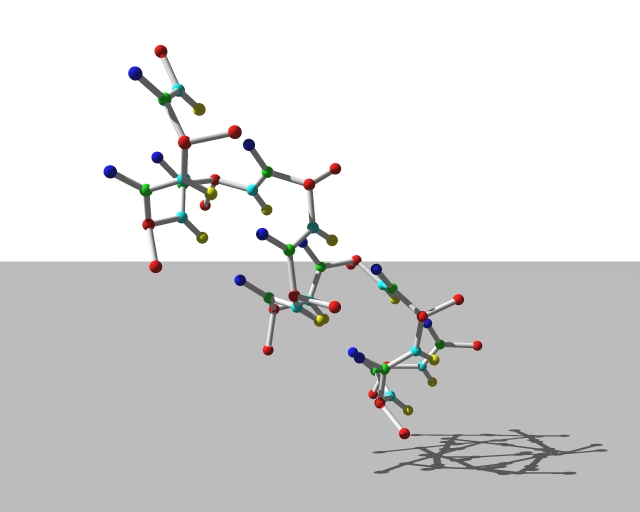
\includegraphics[width=7.5cm]{alanin_66.jpg}}
        \end{minipage} 
        \hfill
       \begin{minipage}[htb]{8cm}
   \centerline{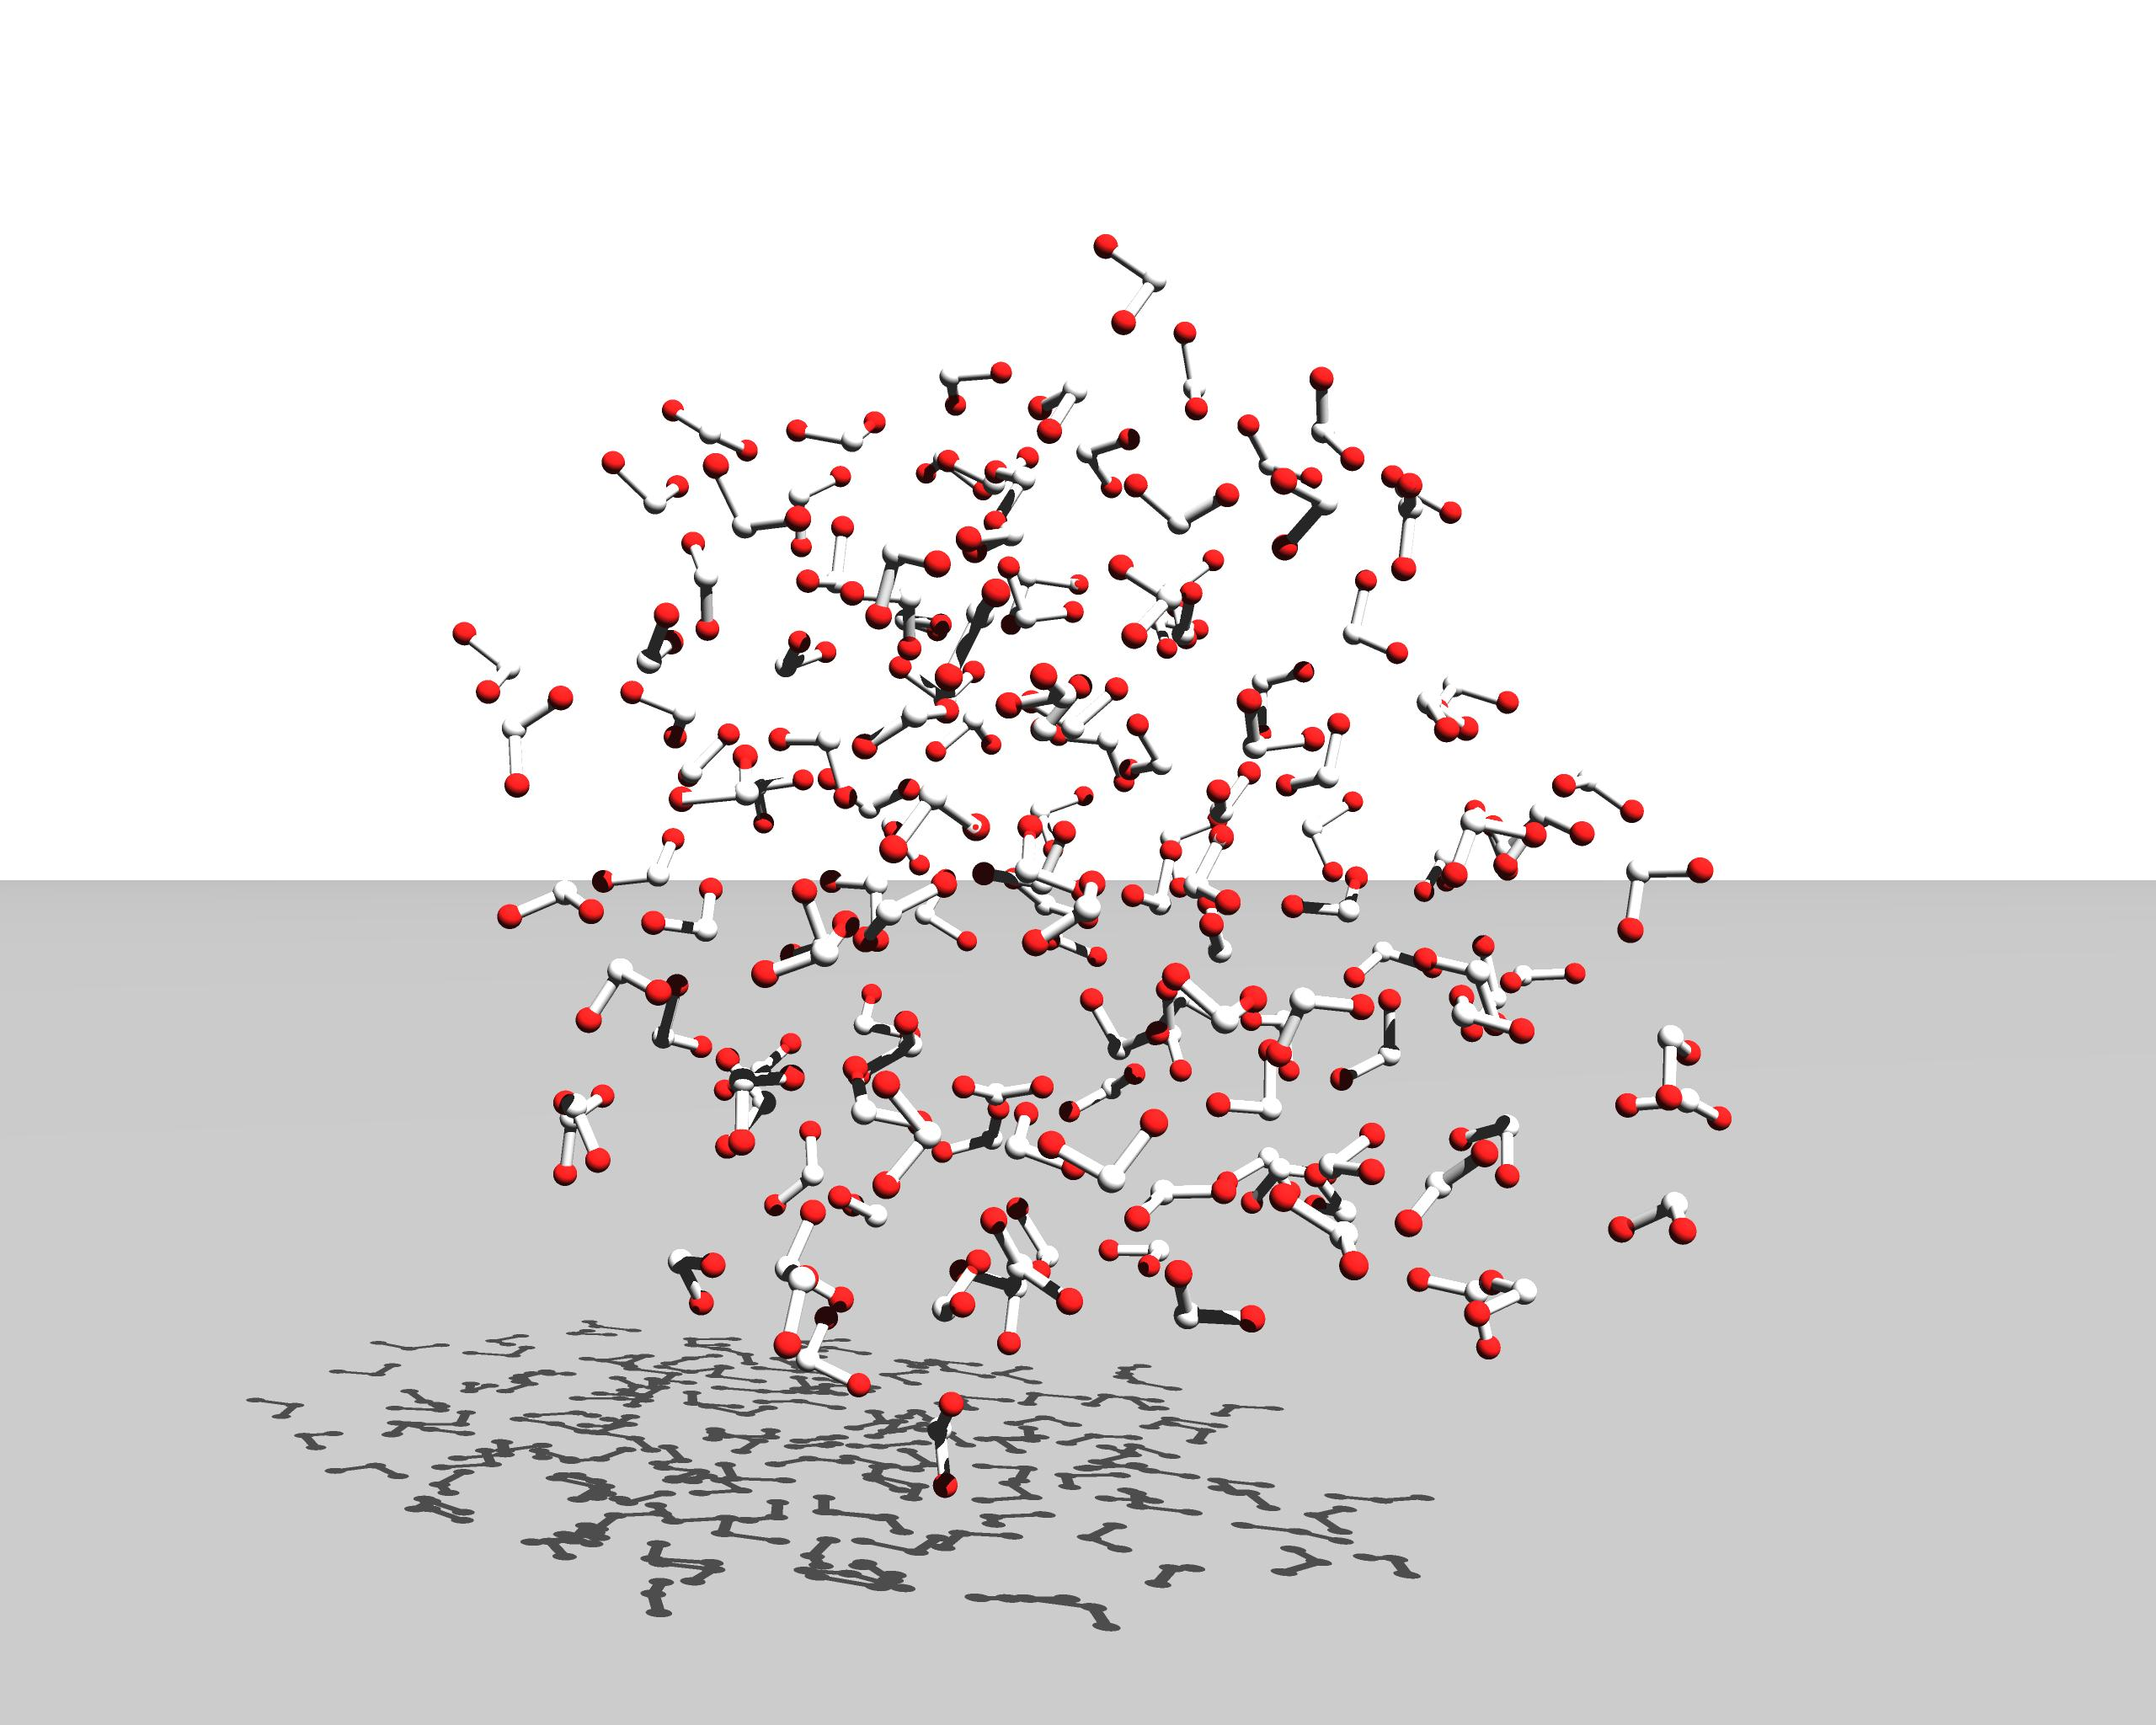
\includegraphics[width=7.5cm]{water_423.jpg}}
        \end{minipage}
        \caption{{\bf Left:} alanin 66 \label{fig:alanin}, 
                 {\bf right:} 10 \AA{ }diameter water droplet.\label{fig:water423}}
\end{figure}
%%%%%%%%%%%%%%%%%%%%%%%%%%%%%%%%%%%%%%%%%%%%%%%%%%%%%%%%%%%%%%%%%%%%%%%%%
\section{Alanin Configuration File with Leapfrog Integrator}
\label{sec:alanin}

Following is an example of a configuration file for the protein
molecule alanin (Fig.\ref{fig:alanin}) .  In this case, \ProtoMol\ will run 10000 steps
starting at time 0, and random velocities will be generated based on
the initial temperature of 300.0 and the random seed of 1234.  A cubic
cell manager is used (this must be true) with a cell size of 6.5.
Output files, in this case just an all energies file and a DCD
trajectory file will be written every 100 timesteps.  Also a final PDB
position and velocity file will be written. The initial
parameter file alanin.par uses the newer CHARMM format.  Vacuum
boundary conditions are present, and the integrator is a
single-timestep leapfrog integrator, with all bonded and two nonbonded
forces present.  The van der Waals and electrostatic forces both use a
nonbonded cutoff algorithm and have cutoffs at 6.5.  The switching
function for the van der Waals potential function makes the second
derivative continuous at the cutoff point, while the electrostatic
potential function has a continuous first derivative due to its
switching function.  The switchon option has been used for van der
Waals (recall that it can only be used with the C2 switching
function). 
\small
\begin{verbatim}
   temperature 300.0
   firststep 0
   numsteps 10000
   cellsize 6.5
   outputfreq 100
   seed 1234
   posfile alanin.pdb
   psffile alanin.psf
   parfile alanin.par
   finpdbposfile alanin.out.pos.pdb
   finXYZvelfile alanin.out.vel.pdb
   DCDfile alanin.out.dcd
   allenergiesfile alanin.out.energy
   boundaryConditions vacuum
   cellManager Cubic
   Integrator {
       level 0 Leapfrog {
                timestep 1
         force Improper
         force Dihedral
         force Bond
         force Angle
         force LennardJones
                  -algorithm NonbondedCutoff
                  -switchingFunction C2
           -switchon 1.0
                  -cutoff 12
         force Coulomb
                  -algorithm NonbondedCutoff
                  -switchingFunction C1
                  -cutoff 12
       }
   }
\end{verbatim}
\normalsize

%%%%%%%%%%%%%%%%%%%%%%%%%%%%%%%%%%%%%%%%%%%%%%%%%%%%%%%%%%%%%%%%%%%%%%%%%
\section{20 \AA{ }diameter water droplet With A Two-Level Integration
  Scheme}

This sample of water (Fig.\ref{fig:water423}) is being run using a two-level integration scheme,
starting with an MTS Impulse Integrator with a cycle length of 5
and finishing with an STS LeapFrog Integrator that has a timestep of
1.0.  The initial temperature is 300 and the first timestep is 0, and
the simulation will be run for 50 steps.  Note the cubic cell manager
and periodic boundary conditions, and that all cell basis vectors have
been provided. Output files, however, will be written,
including a DCD trajectory file and an all energies file, every 10
steps.  
Note that all
necessary initial data files have been provided.
Once again, for the level 1 integrator the Coulombic interaction is computed using
Ewald~\cite{Ewal21,dePS80a} summation. 
\clearpage
\small
\begin{verbatim}
temperature 300.0
firststep 0

numsteps 50

cellsize 6.5

outputfreq 10
seed 1234

posfile equil298K_01.pos.pdb
velfile equil298K_01.vel.pdb

psffile equil298K_01.psf
parfile equil298K_01.par

ALLENERGIESFILE   equil298K_01.out.energies

cellBasisVector1     25.0 0.0 0.0
cellBasisVector2     0.0 25.0 0.0
cellBasisVector3     0.0 0.0 25.0
cellorigin           0.0 0.0  0.0

boundaryConditions Periodic
cellManager Cubic

Integrator {

  level 1 Impulse {
        cyclelength 4
    force Coulomb -algorithm FullEwald -reciprocal
  }
  level 0 Leapfrog {
        timestep 1.0
    force Coulomb -algorithm FullEwald -correction -real
    force Bond, Angle
    force LennardJones
          -algorithm NonbondedCutoff
          -switchingFunction C2
          -cutoff 6.5
      -switchon 0.1
  }
}

\end{verbatim}
\normalsize

%%%%%%%%%%%%%%%%%%%%%%%%%%%%%%%%%%%%%%%%%%%%%%%%%%%%%%%%%%%%%%%%%%%%%%%%%
\section{BPTI with Hybrid Monte Carlo Sampling}

Here is an example of the Hybrid Monte Carlo algorithm used to sample
a BPTI molecule - a 2-level Hybrid Monte Carlo MTS integrator is used.
Once again, the initial timestep is at time 0, but the number of
timesteps to run this time is 100.  1-2 exclusions are desired, and
the cellsize is once again 6.5. Initial temperature has been specified
to be 300 to initialize with random velocities. 
There are now however periodic
boundary conditions, and as a result three cell basis vectors along
with a cell origin are required.  Output files will be written to
every 10 timesteps - this time they include XYZ position and
trajectory files, a DCD trajectory file, and
energies file (thus there will be 10 different energy files
generated - one for each type of energy).  
Note that a final
XYZ position file will be written 
since dofinxyzvelfile is set to
``yes''.  
 Since commotion is set to ``yes'',
center of mass motion will be removed when calculating velocities.
Once again notice the cubic cell manager, and also notice that the
HMCIntegrator does not have forces.  The integrator will run 5 Hybrid
Monte Carlo cycles, with a cycle length of 10 and 50 warm-up cycles,
at a temperature of 300 K.  Four bonded forces (bond, angle, improper,
dihedral) are present, and one nonbonded (FullEwald, the Coulomb force
solved for using Ewald summation).
\small
\begin{verbatim}
  temperature 300
   firststep 0
   numsteps 100
   exclude 1-2
   cellsize 6.5
   cellbasisvector1  32.0    0    0
   cellbasisvector2     0 32.0    0
   cellbasisvector3     0    0 32.0
   cellorigin           0    0    0
   outputfreq 10
   posfile ../data/bpti.pdb
   psffile ../data/bpti.psf
   parfile ../data/bpti.par
   finxyzposfile bpti.out.pos.xyz
   finxyzvelfile bpti.out.vel.xyz
   dofinxyzvelfile yes
   xyzposfile bpti.out.trajectory.pos.xyz
   dcdfile bpti.out.dcd
   allenergiesfile bpti.out.energy
   boundaryConditions Periodic
   commotion yes
   cellManager Cubic
   Integrator {
         level 1 HybridMC {
                 cyclelength 10
                 warmupcycles 50
                 temperature 300.0
      }
        level 0 PLeapFrog {
                 timestep 1
         force Bond, Angle, Dihedral, Improper
         force Coulomb
            -algorithm FullEwald
            -real
            -reciprocal
            -correction
      }
   }


\end{verbatim}
\normalsize


\section{Shadow Hybrid Monte Carlo}
Here is an example of Shadow Hybrid Monte Carlo(SHMC) algorithm using the BPTI molecule-a 2 level 
ShadowHMC integrator is used. The acceptance rate of Hybrid Monte Carlo techniqye decreases exponentiall with 
increasing timestep $\delta{t}$ and $N$, the system size. SHMC is a generalizations of HMC technique that samples
form a p.~d.~f. in all phase space. It achieves an asymptotic speedup of $O({N^{1 \over 4}})$ over Hybrid 
Monte Carlo.
The initial timestep is 0 and the total number of timesteps
to simulate is 10. ShadowHMC takes as input 4 parameters. The {\it temperature} is the simulation
temperature. The seed initializes the random number generator. Like HMC, SHMC uses random number
generator drand(). SHMC needs a tuning parameter $c$ to indicate the divergence between shadow and
total energy. SHMC requires the integrator to be symplectic in order to compute shadow hamiltonian.
That is Verlet/Leapfrog is used as innner integrator. 
The cyclelength specifies the number of steps before the energy difference is computed
and the metropolis criteria is checked. Here it is 25. 
The order specifies the order of the accuracy of the shadow hamiltonian. In \ProtoMol\
, we have only 2 options are available for order, namely $4$ and $8$.
Please see \cite{IzHa04} for further details.

\small
\begin{verbatim}
debug 0
numsteps 10
firststep 0
                                                                                                                   
seed 7536031
                                                                                                                   
posfile bpti.pdb
psffile bpti.psf
parfile bpti.par
temperature 300
                                                                                                                   
outputfreq 1
                                                                                                                   
allenergiesfile bpti.out.energies.shmc
                                                                                                                   
boundaryConditions Periodic
# cellBasisVector1 64.32 0 0
# cellBasisVector2 0 51.167 0
# cellBasisVector3 0 0 51.272
                                                                                                                   
cellManager Cubic
cellsize 4
                                                                                                                   
# removeLinearMomentum  1
# removeAngularMomentum 1
shadowEnergy true
                                                                                                                   
                                                                                                                   
Integrator {
                                                                                                                   
    level 1 ShadowHMC {
                                                                                                                   
        temperature 300
        cyclelength 25
        order 8
        c 0
                                                                                                                   
    }
    level 0 Leapfrog {
                                                                                                                   
        timestep 0.5
                                                                                                                   
        force Improper
        force Dihedral
        force Bond
        force Angle
                                                                                                                   
        force Coulomb
             -algorithm NonbondedSimpleFull
                                                                                                                   
        force LennardJones
             -algorithm NonbondedSimpleFull
                                                                                                                   
    }                                                                                                                   
}
\end{verbatim}
\normalsize

\section{Langevin Impulse}
Here is an example of Langevin Impulse integrator \cite{SkIz02} using united-atom butane. 
The temperature is
the target temperature of the molecule/subsystem. Gamma specifies the collision parameter
or the damping constant. The {\textit NonbondedSimpleFull} option specifies
that the direct method is used to compute non-bonded interactions with no cutoff.
This works only for non-periodic boundary conditions. \ProtoMol\ 2.0.3 comes with a feature
where one can output the dihedral angle values in a file. The phrase dihedralsfile specifies
the filename where dihedral angle values are recorded in radians. Of course , you'll have to set
the dodihedralsfile flag to make it work. dihedralsIndex specifies the index of the dihedral. This
index specifies the order of the dihedral angle in psf file which you are interested in. In this example,
we are using United-atom butane and there is only one dihedral, with index 0. To record multiple torsion
angle one can use the dihedralsSetfile flag to specify an input filename where one can list the dihedral 
indices, one in each line. Note that dihedralsSet flag should be set in order for \ProtoMol\ to take multiple
dihedral indices as input.

\small
\begin{verbatim}
temperature 300
firststep 0

numsteps 500

cellsize 5

outputfreq 10

posfile UA_butane.pdb
psffile UA_butane.psf
parfile UA_butane.par

allenergiesfile ua_butane.lang.out.energy

boundaryConditions vacuum

cellManager Cubic

dodihedralsfile true
dihedralFileOutputFreq 1
dihedralsfile ua_butane.lang.out.dihedrals
dihedralsIndex 0
dihedralsSet false
dihedralsSetfile testset18

Integrator {
  level 0 LangevinImpulse {
    timestep 1.0
    temperature 300
    gamma 7000
    seed 0
    force Bond
    force Angle
    force Dihedral
    force Improper
    force LennardJones Coulomb
      -algorithm NonbondedSimpleFull
  }
}
\end{verbatim}
\normalsize
%%%%%%%%%%%%%%%%%%%%%%%%%%%%%%%%%%%%%%%%%%%%%%%%%%%%%%%%%%%%%%%%%%%%%%%%%

%%%%%%%%%%%%%%%%%%%%%%%%%%%%%%%%%%%%%%%%%%%%%%%%%%%%%%%%%%%%%%%%%%%%%%%%%
\section{Interaction of \ProtoMol\ with VMD}

You may start VMD normally before you begin running the desired
simulation to be viewed in \ProtoMol.  Select the ``molecule'' option
from the main window, and in the resulting molecule window select
``Load From Files''.  Then in the files window that opens, under the
menu ``Molecule File Types'' select psf and pdb, then write the full
pathnames of the PSF and PDB files used in the simulation that will be
run in the provided spaces.  Now VMD has the initial state of the
molecule to be simulated. \\

Next, in the configuration file that will be used, make sure there is
a Haptic force in the integrator.  Check to see that a positive
nonzero value is supplied for the ``-wait'' value under the haptic
force.  This will force \ProtoMol\ to wait some time for an IMD
connection, 100 would be a decent value so that you have time to set
VMD to simulate.  Also note the port number, which will be used
later.\\

Now run \ProtoMol.  It should display ``Waiting for IMD
connection.....'' after a short time.  At this point, go to the VMD
console window and type ``\ttsmall{imd connect <hostname> <port
number>}'', where \ttsmall{<hostname>} is the name of the
machine that \ProtoMol\ is running on and \ttsmall{<port number>}
is the port number value specified in the configuration file that is
being used.\\

At this point, VMD will view the molecule throughout the simulation as
\ProtoMol\ runs.  Also from the VMD window IMD commands can be run that
will send messages to \ProtoMol.  For example, typing\\ ``\ttsmall{imd
trate <integer value>}'' will change the transmission rate for
information from \ProtoMol\ to VMD.\\

As an example, let us return to the integrator section of the alanin configuration file from section \ref{sec:alanin}:\\

\begin{verbatim}        
Integrator {
       level 0 Leapfrog {
                timestep 1
         force Improper 
         force Dihedral
         force Bond
         force Angle 
         force LennardJones
                  -algorithm NonbondedCutoff
                  -switchingFunction C2
           -switchon 0.1
                  -cutoff 12
         force Coulomb
                  -algorithm NonbondedCutoff
                  -switchingFunction C1
                  -cutoff 12
         force Haptic
           -port 2001
           -trate 1
           -timeout 1000
           -step_inc 100
           -wait 100
       }
   }
\end{verbatim}        

The only area that counts as far as the VMD simulation is concerned is
the ``\ttsmall{force Haptic}'' section at the end.  Notice first that
a \ttsmall{-wait} value is given that is greater than zero, thus
\ProtoMol\ will wait for an IMD connection, which is what we want.  The
port ID is 2001.  The other three values are IMD variables. \\ 

In this case as soon as \ProtoMol\ begins waiting for the IMD
connection, a user would type\\ ``\ttsmall{imd connect <name of the
    machine on which \ProtoMol\ is running> 2001}'' and the visual
simulation will begin.  Now the user can run IMD commands in the IMD
window while the simulation is running.
\begin{figure}[htb]
   \centerline{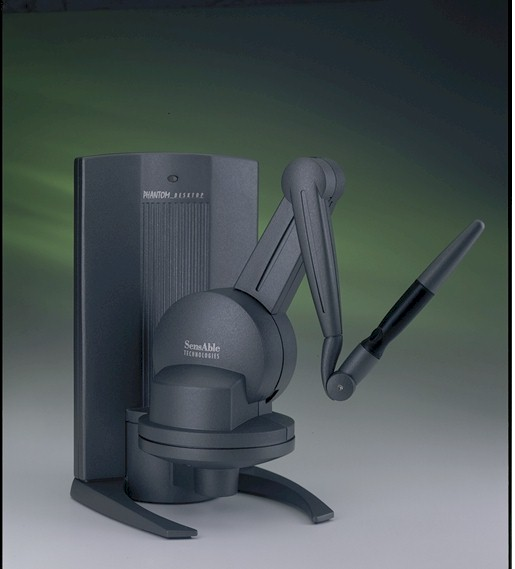
\includegraphics[width=8cm]{hapticdevice.jpg}}
    \caption{ PHANTOM Desktop$^{\mbox{TM}}$ Haptic Device.  \label{fig:hapticdevice}}
\end{figure}


\begin{appendix}
%%%%%%%%%%%%%%%%%%%%%%%%%%%%%%%%%%%%%%%%%%%%%%%%%%%%%%%%%%%%%%%%%%%%%%%%%
\chapter{Contact Information}
                                                                                               
The best contact path for licensing issues is by e-mail to
{\it protomol@cse.nd.edu} or send correspondence to: \\ \\
\ProtoMol\ Team\\
c/o Prof. Jes\'{u}s A. Izaguirre\\
Laboratory for Computational Life Sciences\\
Department of Computer Science and Engineering\\
University of Notre Dame\\
384 Fitzpatrick Hall of Engineering\\
Notre Dame, Indiana 46556 USA
                                                                                               
%%%%%%%%%%%%%%%%%%%%%%%%%%%%%%%%%%%%%%%%%%%%%%%%%%%%%%%%%%%%%%%%%%%%%%%%%
\end{appendix}


\bibliographystyle{abbrv}
\bibliography{lcls}
\end{document}
